%versi 2 (8-10-2016)
\chapter{Landasan Teori}
\label{chap:teori}


 
Pada bab ini akan dibahas mengenai dasar teori yang digunakan pada penyusunan tugas akhir. Pembahasan pertama mencakup hal-hal yang berkaitan dengan pengertian kewirausahaan dari umum sampai khusus yaitu kewirausahaan menurut GEM. Pembahasan kedua yaitu tentang teori dan aplikasi dari CA (Cellular Automata) khususnya tentang ECA (Entrepreneur Cellular Automata). Pembahasan terakhir tentang hal-hal lain yang mendukung implementasi perangkat lunak seperti... 


\section{Arti Kewirausahaan}
\label{sec:artiwirausaha}

\graphicspath{{images/}}

Secara umum arti kewirausahaan merupakan suatu proses dalam mengerjakan sesuatu yang baru dan berbeda yang bermanfaat bagi orang lain atau diri sendiri. Orang yang melakukan proses kewirausahaan adalah wirausaha. Ciri-ciri wirausaha antara lain yaitu berani mengambil risiko, memiliki semangat dan kemauan keras, memiliki jiwa pemimpin, dsb. Tujuan wirausaha sendiri yaitu menciptakan lapangan kerja yang baru dan meningkatkan jumlah para wirausaha di suatu negara.


Kewirausahaan menurut GEM merupakan proses yang terdiri dari fase-fase berbeda mulai dari niat mendirikan suatu usaha, menjalankan suatu usaha baru atau sudah berdiri, sampai dengan penghentian sebuah usaha. Proses ini dimulai dengan keterlibatan individu yang berpotensi untuk menjadi wirausaha, yaitu mereka yang percaya bahwa mereka mempunyai kemampuan untuk memulai suatu usaha, individu yang melihat kesempatan untuk berwirausaha dan individu yang tidak takut gagal dalam memulai suatu usaha.
\begin{figure} 
	\centering  
	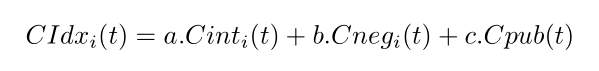
\includegraphics[width=14cm, height=6cm]{Capture}  
	\caption[Fase Wirausaha]{Fase Wirausaha} 
	\label{fig:artiwirausaha} 
\end{figure}

Pada gambar \ref{fig:artiwirausaha}, dijelaskan fase pertama dari ilustrasi GEM adalah wirausaha \textit{nascent}. Wirausaha \textit{nascent} adalah mereka yang telah memulai suatu usaha baru namun masih sangat dini (< 3 bulan). Setelah lebih dari tiga bulan, wirausaha \textit{nascent} ini disebut Pemilik Usaha Baru (\textit{new business owner}). Fase ini dijalani sampai individu tersebut telah tiga setengah tahun tahun terlibat dalam kewirausahaan. Kegiatan pada fase wirausaha \textit{nascent} dan pemilik usaha baru masuk kedalam kelompok Total Early Stage Entrepreneurial Activity (TEA). Fase selanjutnya adalah fase dimana wirausaha disebut sebagai Pemilik Usaha Mapan (\textit{owner-manager of an established business}). 

GEM mempertimbangkan beberapa indikator yang mempengaruhi berlangsungnya kewirausahaan di suatu negara yaitu \textit{Entrepreneurial Intention}, \textit{Fear of Failure}, \textit{perceived opportunities} dan \textit{Perceived Capabilities}. \textit{Entrepreneurial Intention} mendeskripsikan presentase dari populasi berusia 18-64 yang bertekad untuk mendirikan suatu usaha dalam waktu tiga tahun kedepan. \textit{Fear of Failure} mendeskripsikan presentase dari populasi berusia 18-64 dengan  yang positif yang mengindikasikan bahwa takutnya gagal dalam menghambat mereka dalam mendirikan suatu usaha. \textit{Perceived Opportunities} mendeskripsikan persentase dari populasi berusia 18-64 yang melihat kesempatan bagus untuk memulai suatu usaha di daerah tempat tinggal mereka. \textit{Perceived Capabilities} mendeskripsikan persentase dari populasi berusia 18-64 yang merasa mempunyai kemampuan dan pengetahuan yang cukup untuk mendirikan suatu usaha.



 
